\chapter{Kilika}

\begin{enumerate}
  \item \sd\ on exiting the boat, go up and left, \sd. \skippablefmv[2:00], (press Start immediately after skip) \sd
  \item Exit inn, go right to \wakka, \sd. Go left and up to Kilika Woods, \sd
\end{enumerate}
\begin{battle}{Lancet Tutorial}
  \begin{itemize}
    \item \sd
          \kimahrif Lancet
          \tidusf Attack
          \switch{anyone}{\yuna}
          \yunaf Attack
          \luluf Fire
  \end{itemize}
\end{battle}
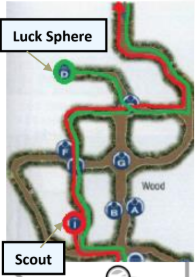
\includegraphics{graphics/kilikamap}
\begin{enumerate}[resume]
  \item Go left and up the hidden path, \pickup{Scout}
\end{enumerate}
\begin{spheregrid}
  \begin{itemize}
    \tidusf Go to Flee, learn Flee and Agility +1
  \end{itemize}
  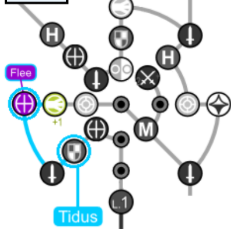
\includegraphics{graphics/tidusflee}
\end{spheregrid}
\begin{equip}
  \begin{itemize}
    \wakkaf Scout
    \item \textit{If you got the Ice Brand:}
          \begin{itemize}
            \tidusf Ice Brand
          \end{itemize}
  \end{itemize}
\end{equip}
\begin{enumerate}[resume]
  \item \formation{\tidus}{\yuna}{\wakka}
  \item Continue up the hidden path, following the map.
\end{enumerate}
\begin{encounters}
  \begin{itemize}
    \item Killer Bee:
          \begin{itemize}
            \wakkaf Attack
            \luluf Blizzard
          \end{itemize}
    \item Dinonix: \tidus\ Attack
    \item Yellow Element: \lulu\ Water
    \item Ragora: Flee
  \end{itemize}
  Keep track of Speed Spheres, need 17 over the course of the run. Need about 45-55 AP on \tidus, which is about 6 kills these encounters.
\end{encounters}
\begin{enumerate}[resume]
  \item\save,  \sd
  \item \formation{\tidus}{\yuna}{\wakka}
  \item \save
\end{enumerate}
\begin{battle}[3000]{Sinspawn Geneaux}
  \begin{itemize}
    \item \textit{If \tidus\ is going before \yuna:}
          \begin{itemize}
            \tidusf Attack Main Body
            \summon{\valefor}
            \valeforf Energy Blast \od
            \valeforf Fire x4-5
          \end{itemize}
    \item \textit{Else:}
          \begin{itemize}
            \switch{\yuna}{\kimahri}
            \kimahrif Attack Main Body
            \tidusf Defend
            \switch{anyone}{\yuna}
            \summon{\valefor}
            \valeforf Energy Blast \od
            \valeforf Fire x4
          \end{itemize}
  \end{itemize}
\end{battle}
\begin{enumerate}[resume]
  \item \sd\ on stone steps and temple. go into temple. Walk up to \wakka\ and Pray. \sd\ inside temple and go up steps. Wait for life and \sd.
\end{enumerate}
\begin{trial}
  \begin{itemize}
    \item Take the sphere from the pedestal
    \item Place into the door, take it off of the door.
    \item Place sphere into the next door, take the sphere back.
    \item Place the sphere into the right holder
    \item Touch glpyh
    \item Take the sphere from the next room
    \item Place it into the left holder
    \item Take the glyph sphere from the pedestal
    \item Place it in the Fire Room
    \item Take the sphere that you put into the right holder
    \item Use it to open the door in the Fire Room
    \item Take the sphere off the door
    \item Enter the Fayth room
  \end{itemize}
\end{trial}
\begin{enumerate}[resume]
  \item In Fayth room, \sd, speak to \wakka\ first. Try to leave room, \sd, name \ifrit
  \item Hold down to exit temple, \cs[0:40], \sd
  \item Go south through Kilika Woods, take the left path and \pickup{Luck Sphere}, referencing map.
  \item Exit Kilika Woods same way that you entered, treating fights the same way as above.
  \item Go down and right to S.S. Winno. \sd
\end{enumerate}